\documentclass[12pt]{article}

\usepackage[italian]{babel} 
\usepackage[utf8x]{inputenc}
\usepackage{graphicx}
\usepackage{cleveref}
\usepackage{wrapfig}

\graphicspath{ {images/} }

\pagestyle{headings}
\title{R2Pi0}
\author{
  Tosatto Davide
  \and
  Riccardo Grespan
}

\newcommand{\cbegin}{‘‘}
\newcommand{\cend}{’’}
\newcommand{\imgsz}{0.3\textwidth}

\makeindex

\begin{document} 
\maketitle
\newpage
\tableofcontents
\newpage

\section{Obiettivi del progetto}
L'obiettivo del progetto è di creare una riproduzione in scala di R2-D2, noto personaggio robotico della serie di Star Wars.

\begin{figure}[h]
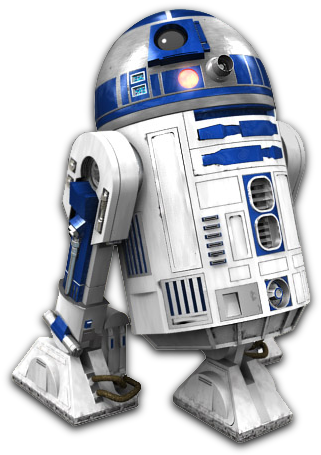
\includegraphics[width=\imgsz]{R2D2}
\centering
\caption{R2D2}
\label{fig:R2D2}
\end{figure}

La ricostruzione comprende:
\begin{enumerate}
\item movimento sul piano attraverso ruote (come nel film)
\item riproduzione di suoni simili a quelli originali attraverso un buzzer, per dare quel tocco di retro che non guasta mai
\item luci led e finto proiettore, comunque emulato da un led
\item rilevamento degli ostacoli e corrispondente arrabbiatura del robot se lo mandiamo a tutta velocità verso uno di essi
\item funzione follow che gli fa mantenere una certa distanza dall'oggetto (o dalla persona) che lo precede
\item un rudimentale controllo vocale
\item esoscheletro in carta che riproduce le fattezze del robot
\end{enumerate}

Questa prima versione non avrà la possibilità di ruotare la testa e cambiare inclinazione, questo per mancanza di tempo e di componenti (ulteriori motori, ulteriori driver, contatti girevoli per le luci che stanno sulla testa)
 
\section{Componenti e scelte progettuali}
\subsection{Scheda di controllo}
Iniziamo dal cuore del progetto: \emph{la scheda di controllo}.

Le opzioni erano sostanzialmente due: Raspberry Pi0 o Arduino Uno.

\begin{figure}[h]
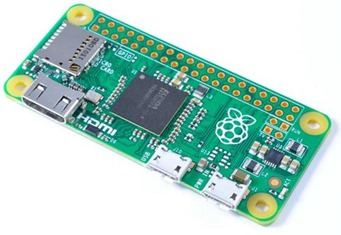
\includegraphics[width=\imgsz]{rpi0}
\centering
\caption{Raspberry Pi0}
\label{fig:rpi0}
\end{figure}

\begin{figure}[h]
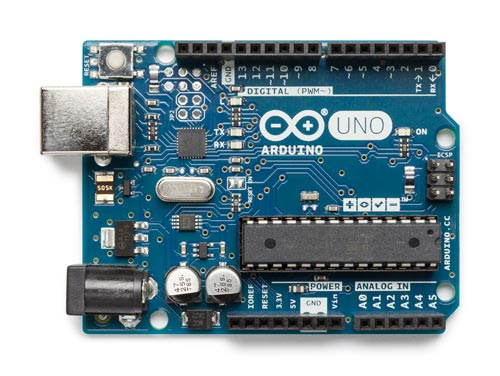
\includegraphics[width=\imgsz]{Uno}
\centering
\caption{Arduino Uno}
\label{fig:uno}
\end{figure}

Per la maggior parte dei compiti le due schede erano sostanzialmente intercambiabili, in particolare:
\begin{enumerate}
\item \emph{GPIO - General Purpose Input Output}: entrambi i dispositivi hanno tutte le interfacce che ci servono, ossia qualche I/O digitale e uscite PWM. Entrambi non possono dare in uscita elevate correnti, ma questo non importa perché il controllo di ogni componente è sempre mediato da transistor esterni;
\item \emph{Alimentazione}: entrambi i dispositivi possono essere alimentati da usb, rendendo quindi possibile l'uso di una normale batteria esterna da telefono per l'alimentazione;
\item \emph{Potenza di calcolo}: entrambi i dispositivi in esame hanno la potenza di calcolo necessaria per svolgere ognuno dei compiti necessari agli scopi del progetto.
\end{enumerate} 

Le seguenti motivazioni ci hanno fatto propendere per Raspberry Pi0:
\begin{enumerate}
\item \emph{Semplicità di sviluppo}: grazie al fatto di avere a disposizione un sistema operativo completo, possiamo utilizzare linguaggi di più alto livello rispetto al C fornito da Arduino. Questo ci permette di creare codice meglio organizzato e più facilmente espandibile in futuro. La nostra scelta per il linguaggio è ricaduta su \emph{Python}, in quanto semplice, conciso ed efficace;
\item \emph{Memoria a disposizione}: grazie alla memoria disponibile, sensibilmente superiore a quella di Arduino, ci è permesso di integrare più suoni. Inoltre, in futuro, sarà sempre possibile migliorare la qualità degli stessi.
\item \emph{Facilità di connessione}: Raspberry Pi0 risulta più facile da connettere al mondo in quanto basta collegare un adattatore wifi o bluetooth all'USB. Arduino invece richiede appositi shield, costosi e non utilizzabili su altre schede, almeno non senza opportune modifiche
\item \emph{Prezzo}: Raspberry Pi0 costa 5\$, molto meno di un Arduino, e, nonostante questo, offre infinite possibilità in più in quanto propone un sistema completo di tutto.
\end{enumerate}

Certo Raspberry Pi0 ha dalla sua un grande svantaggio: il consumo.

Arduino a vuoto consuma circa 50mA, mentre Raspberry Pi0 arriva a 65mA in idle, ma si alza parecchio se il carico di lavoro aumenta, questo perchè il processore di Raspberry Pi0 è molto più performante di quello di Arduino, inoltre, montando un sistema operativo completo, Raspberry Pi0 ha anche diverso overhead in campo di potenza computazionale e consumo, cosa non trascurabile.

Chiaramente poi i dispositivi di comunicazione comportano un innalzamento dei consumi, ma questo su entrambe le schede.

In conclusione, i vantaggi nell'utilizzo di Raspberry Pi0 ci sono sembrati schiaccianti.

\subsection{Comunicazione}
Anche qui, due opzioni iniziali: Bluetooth o WiFi.

Abbiamo optato per una connessione Bluetooth per i seguenti motivi:
\begin{enumerate}
\item \emph{Consumo}: il Bluetooth risulta avere un consumo energetico inferiore rispetto al WiFi, portandoci ad avere una durata della batteria leggermente superiore (non abbiamo dati precisi)
\item \emph{Semplicità d'uso}: il Bluetooth è pensato per connessioni punto a punto, ossia esattamente la funzione che serve a noi. Il Wifi, invece, non è pensato per quello scopo e quindi relegherebbe all'utilizzo nei soli spazi dotati di rete WiFi oppure alla configurazione di una rete ad-hoc che risulta comunque un'operazione non banale e spesso mal funzionante (soprattutto su Linux)
\end{enumerate}

\section{Schemi circuitali}
\subsection{Controllo motori}
Per il controllo dei motori abbiamo deciso di utilizzare una versione leggermente modificata del ponte H. I nomi dei componenti sono presi da \cref{fig:ponteH}. \'E ovviamente necessario uno di questi circuiti per ogni motore installato.

\begin{figure}[h]
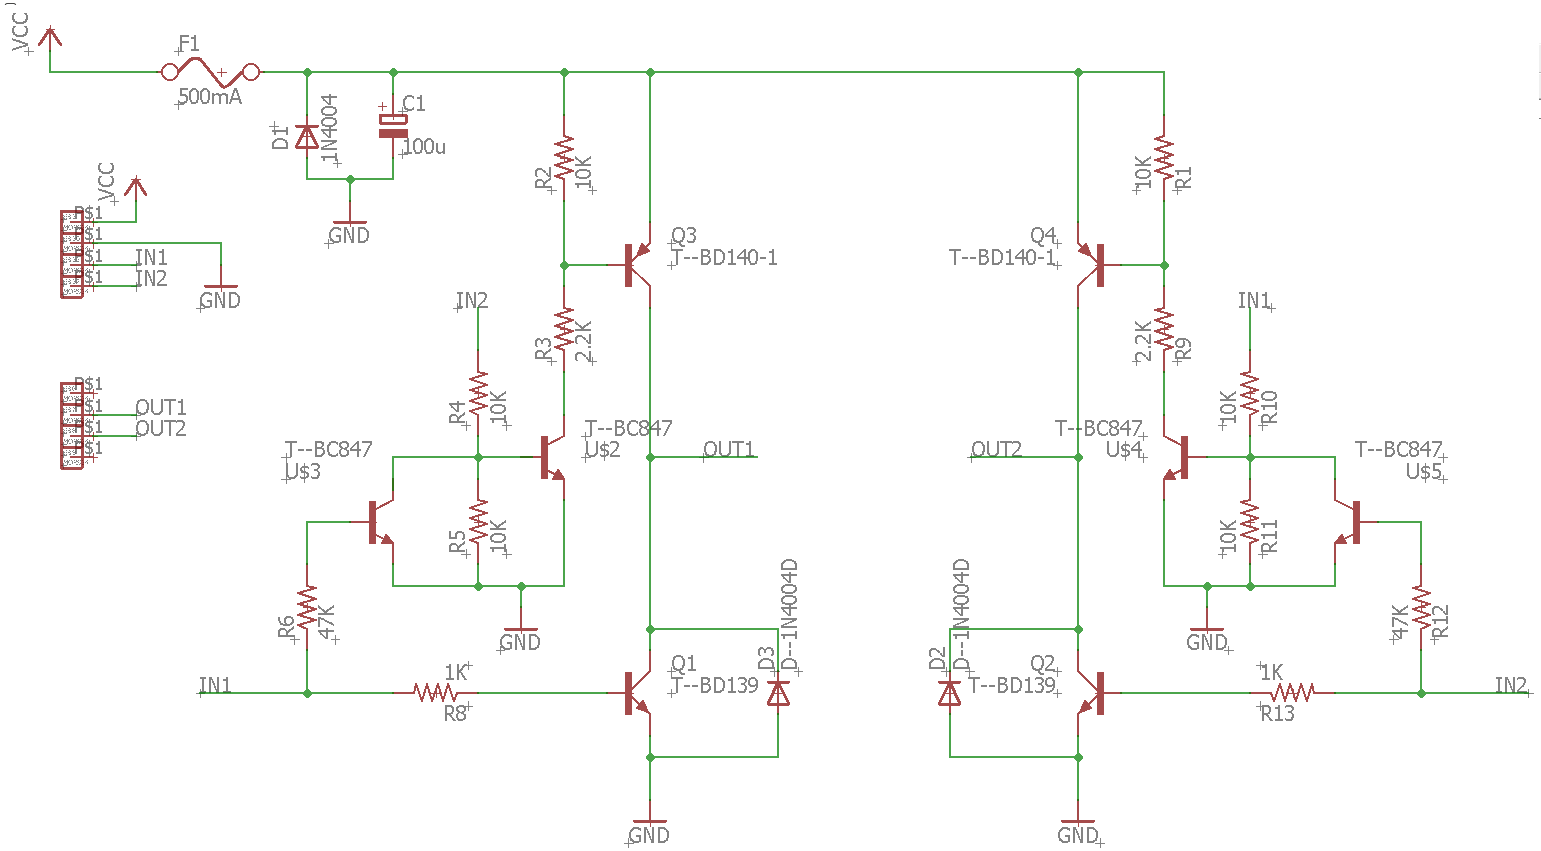
\includegraphics[width=\textwidth]{SchemaH}
\centering
\caption{Schema del circuito di controllo dei circuiti}
\label{fig:ponteH}
\end{figure}

Passiamo alla rapida spiegazione del funzionamento del circuito. Il circuito ha due input: IN1 e IN2. Il comportamento è il seguente:
\begin{enumerate}
\item Se solo uno dei due fra IN1 e IN2 è attivo, nel motore scorre corrente, il verso dipende da quale dei due è alto.
\item Se sia IN1 che IN2 sono a 0, il motore resta completamente scollegato dal circuito, permettendogli di muoversi per inerzia
\item Se sia IN1 che IN2 sono a 1, il motore ha entrambi i terminali a massa. Questo chiude la bobina del motore creando un cortocircuito. Così facendo se si tenta di muovere il motore si originerà all'interno della bobina una corrente che genererà a sua volta un campo magnetico che si opporrà al movimento del motore. Questo ha come risultato un effetto frenante. 
\end{enumerate}

Passiamo alla disamina dei componenti e delle loro funzioni.
Tutti i transistori sono BJT. Questa scelta è stata fatta perché i BJT permettono di fare passare correnti elevate e soprattutto hanno basse cadute di potenziale in saturazione, ossia circa 0.3V tra collettore ed emettitore. Mantenere cadute di potenziale basse è essenziale perché il tutto è alimentato a soli 5V.

I quattro transistor principali di potenza sono Q1, Q2, Q3 e Q4. La circuiteria è fatta in modo tale che né Q1 e Q3, né Q2 e Q4 conducano \emph{mai} insieme. Questo avvenimento infatti produrrebbe un cortocircuito che danneggerebbe il circuito.

Da misurazioni, si è visto che i motori consumano meno di 200mA l'uno, e si è dunque pensato di inserire per sicurezza un fusibile da 500mA, F1, sufficientemente permissivo da far funzionare il motore, ma abbastanza restrittivo per evitare di bruciare l'alimentatore in caso di corto, che comunque, salvo manomissioni, non dovrebbe avvenire.

Abbiamo poi altri quattro transistor che servono ad assicurare l'assenza di corti e ad implementare la funzionalità di cortocircuitare la bobina con entrambi gli ingressi a 1.

La funzione logica realizzata è quella mostrata in tabella \ref{tab:tabFunz}

\begin{table}[h]
\begin{center}


\begin{tabular}{l|l|l|l|l|l}

IN1 & IN2 & Q1 & Q2 & Q3 & Q4 \\
\hline
off & off & off & off & off & off \\
off & on & off & on & on &  off \\
on & off & on & off & off &  on \\
on & on & on & on & off & off


\end{tabular}

\end{center}
\caption{Funzione logica implementata nel circuito}
\label{tab:tabFunz}
\end{table}


\end{document}
